% $Header: /cvsroot/latex-beamer/latex-beamer/solutions/conference-talks/conference-ornate-20min.en.tex,v 1.6 2004/10/07 20:53:08 tantau Exp $

\documentclass{beamer}

% This file is a solution template for:

% - Talk at a conference/colloquium.
% - Talk length is about 20min.
% - Style is ornate.



%
% In principle, this file can be redistributed and/or modified under
% the terms of the GNU Public License, version 2.
%
% However, this file is supposed to be a template to be modified
% for your own needs. For this reason, if you use this file as a
% template and not specifically distribute it as part of a another
% package/program, I grant the extra permission to freely copy and
% modify this file as you see fit and even to delete this copyright
% notice. 


\mode<presentation>
{
  \usetheme{Warsaw}
  % or ...

  \setbeamercovered{transparent}
  % or whatever (possibly just delete it)
}


\usepackage[english]{babel}
% or whatever

\usepackage[latin1]{inputenc}
% or whatever

\usepackage{times}
\usepackage[T1]{fontenc}
% Or whatever. Note that the encoding and the font should match. If T1
% does not look nice, try deleting the line with the fontenc.


\title[Techniques for Fractal Terrain Generation] % (optional, use only with long paper titles)
{Techniques for Fractal Terrain Generation}

%\subtitle
%{Include Only If Paper Has a Subtitle}

\author[K. Bird, T. Dickerson, J. George] 
% (optional, use only with lots of authors)
{A.~Krista Bird \and B.~Thomas Dickerson \and C.~Jessica George}
% - Give the names in the same order as the appear in the paper.
% - Use the \inst{?} command only if the authors have different
%   affiliation.

%\institute[Universities of Somewhere and Elsewhere] % (optional, but mostly needed)
%{
  %\inst{1}%
  %Department of Computer Science\\
  %St. Michael's College
  %\and
  %\inst{2}%
  %Department of Theoretical Philosophy\\
  %Gettysburg College
  %\and
  %\inst{3}
  %Wartburg College
  %\and
  %\inst{4}
  %Pacific University 
  %\and
  %\inst{5}
 % Seattle Pacific University 
%}
% - Use the \inst command only if there are several affiliations.
% - Keep it simple, no one is interested in your street address.

\date[HRUMC] % (optional, should be abbreviation of conference name)
{HRUMC Presentation, 2013}
% - Either use conference name or its abbreviation.
% - Not really informative to the audience, more for people (including
%   yourself) who are reading the slides online

%\subject{Theoretical Computer Science}
% This is only inserted into the PDF information catalog. Can be left
% out. 



% If you have a file called "university-logo-filename.xxx", where xxx
% is a graphic format that can be processed by latex or pdflatex,
% resp., then you can add a logo as follows:

% \pgfdeclareimage[height=0.5cm]{university-logo}{university-logo-filename}
% \logo{\pgfuseimage{university-logo}}



% Delete this, if you do not want the table of contents to pop up at
% the beginning of each subsection:
%\AtBeginSubsection[]
%{
 % \begin{frame}<beamer>
 %   \frametitle{Outline}
 %   \tableofcontents[currentsection,currentsubsection]
 % \end{frame}
%}


% If you wish to uncover everything in a step-wise fashion, uncomment
% the following command: 

%\beamerdefaultoverlayspecification{<+->}


\begin{document}

\begin{frame}
  \titlepage
\end{frame}

\begin{frame}
  \frametitle{Outline}
  \tableofcontents
  % You might wish to add the option [pausesections]
\end{frame}


% Structuring a talk is a difficult task and the following structure
% may not be suitable. Here are some rules that apply for this
% solution: 

% - Exactly two or three sections (other than the summary).
% - At *most* three subsections per section.
% - Talk about 30s to 2min per frame. So there should be between about
%   15 and 30 frames, all told.

% - A conference audience is likely to know very little of what you
%   are going to talk about. So *simplify*!
% - In a 20min talk, getting the main ideas across is hard
%   enough. Leave out details, even if it means being less precise than
%   you think necessary.
% - If you omit details that are vital to the proof/implementation,
%   just say so once. Everybody will be happy with that.

\section{Introduction}
\subsection{What is Fractal Terrain Generation?}

\begin{frame}
  \frametitle{Connecting Fractal Geometry and Terrain}
  %\framesubtitle{Subtitles are optional.}
  % - A title should summarize the slide in an understandable fashion
  %   for anyone how does not follow everything on the slide itself.
  \begin{itemize}
  \item What is fractal geometry?
  \item Benoit Mandlebrot and the length of the British coastline. (Stanger)
  \end{itemize}
  \begin{center}
  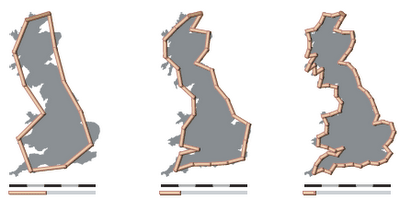
\includegraphics[scale=0.5]{BritainCoastline.png}
  \end{center}
\end{frame}

\begin{frame}
\frametitle{Why are Fractals useful in Generating Landscapes}
\begin{itemize}
\item Self Similar
\item Non-integer dimension
\end{itemize}
\begin{center}
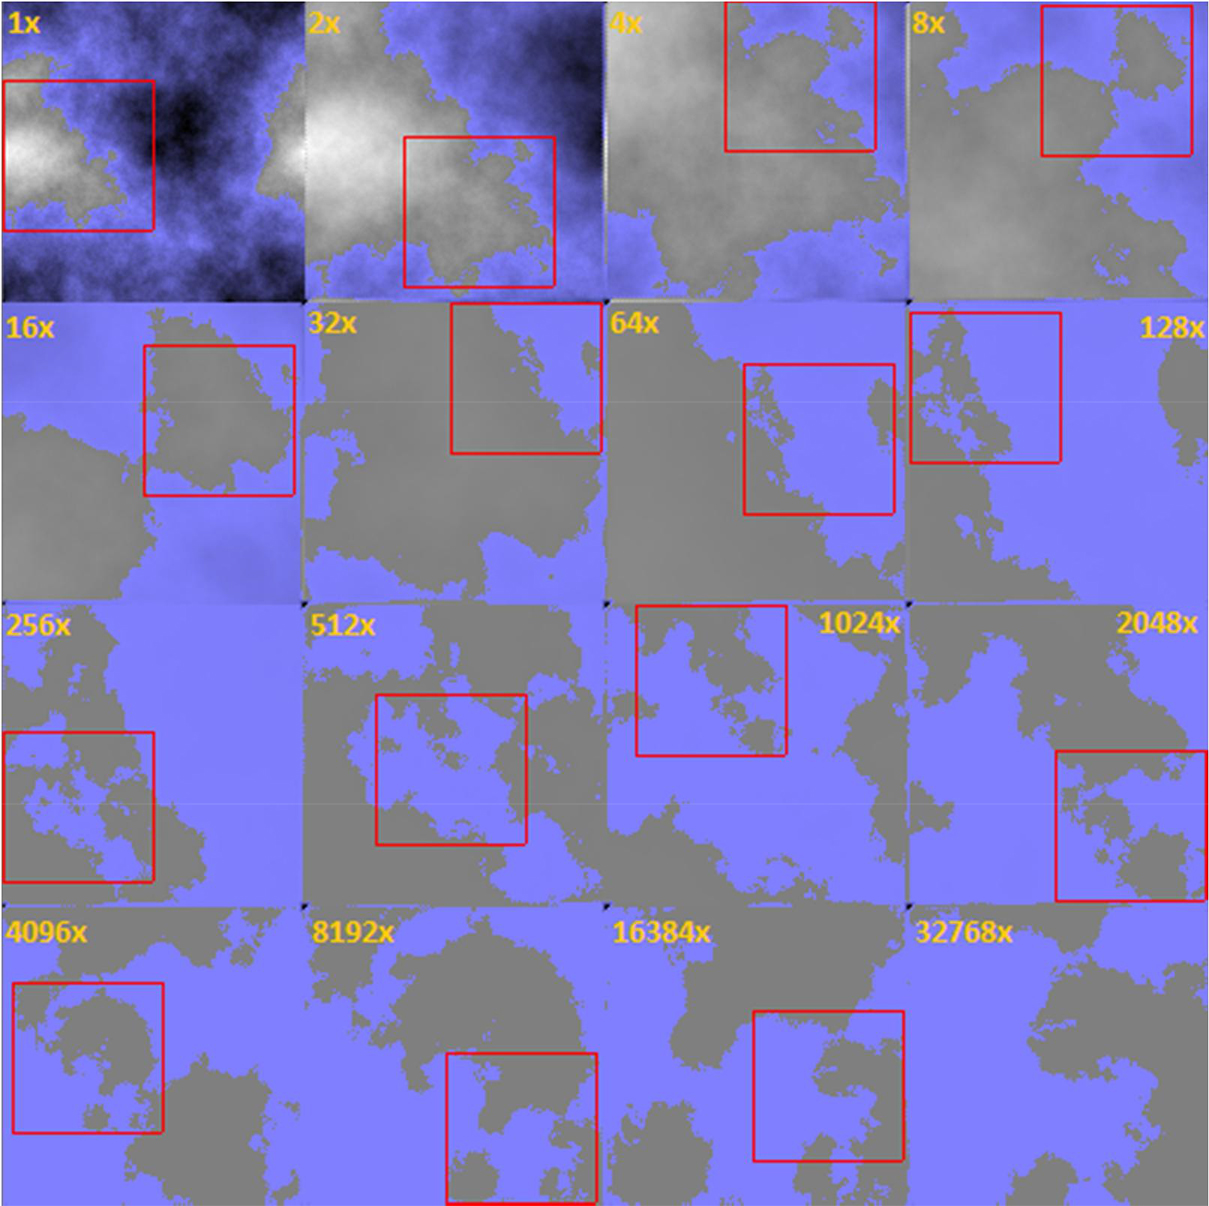
\includegraphics[scale=0.13]{SelfSimilarity.jpg}
\end{center}
\end{frame}


\section{Fractal Terrain Generation Methods}
\subsection{Midpoint Displacement Method}

\begin{frame}
  \frametitle{Midpoint Displacement Method}
\begin{itemize}
 \item Relatively straightforward
 \item Realistic features
\item Begin with a line between two points.
\item The midpoint of this line this then displaced by some random amount in a vertical direction.
\item The midpoints of these two new line segments are then displaced by a random amount in the vertical direction.
\item Repeat until you have reached desired level of detail.
\end{itemize}
\end{frame}

\begin{frame}
\frametitle{Midpoint Displacement (cont.)}
\begin{itemize}
 \item Must be a square with sides of length $2^{N}+1$, so that each sub-square has an exact middle lying on a gridpoint.
 \item $k,k' \in \left\{ 1, 3, \cdots, 2^{N-n}-1 \right\}$
 \item $m \in \left\{ 0, 2, \cdots, 2^{N-n} \right\}$
  \item $n < N$ and $m \in \mathbb{Z}$.
 \item H is a smoothing parameter
 \item A is an amplitude parameter
 \item R is uniform random variable between -1 and 1.
\end{itemize}
\end{frame}

\begin{frame}
\frametitle{Midpoint Displacement (cont.)}
\begin{itemize}
 \item Given a heightfield,
		$T = \left[ \begin{matrix}
		T_{0,0} & \ldots & T_{0,2^{N},} \\
		\vdots  &  \ddots & \vdots \\
		T_{2^{N},0} & \ldots & T_{2^{N},2^{N}}
		\end{matrix} \right]$
 \item Recurrence relations for midpoints:
	%\begin{itemize}
		\item along columns
		
		$T_{k \cdot 2^{n},j \cdot 2^{n}} = \frac{T_{(k+1) \cdot 2^{n},j \cdot 2^{n}} + T_{(k-1) \cdot 2^{n},j \cdot 2^{n}}}{2} + A \cdot R \cdot 2^{-H \cdot n}$,
		\item along rows
		
		$T_{j \cdot 2^{n},k \cdot 2^{n}} = \frac{T_{j \cdot 2^{n},(k+1) \cdot 2^{n}} + T_{j \cdot 2^{n},(k-1) \cdot 2^{n}}}{2} + A \cdot R \cdot 2^{-H \cdot n}$,
		\item and between corners
		
		$T_{k \cdot 2^{n},k' \cdot 2^{n}} = \left(\frac{1}{4}\right)T_{(k-1) \cdot 2^{n},(k'-1) \cdot 2^{n}} + \left(\frac{1}{4}\right)T_{(k-1) \cdot 2^{n},(k'+1) \cdot 2^{n}} + \left(\frac{1}{4}\right)T_{(k+1) \cdot 2^{n},(k'-1) \cdot 2^{n}} + \left(\frac{1}{4}\right)T_{(k+1) \cdot 2^{n},(k'+1) \cdot 2^{n}} + A \cdot R \cdot 2^{-H \cdot n}$
	%\end{itemize}
\end{itemize}
\end{frame}


\begin{frame}
 \frametitle{Diamond Square Algorthim}
\begin{itemize}
\item Variations of the Midpoint Displacement method
\item Midpoint Displacement sometimes leaves square-shaped artifacts in the terrain. 
\item The Diamonds and Squares method attempts to alleviate this by alternating calculated values to square and diamond patterned midpoints. 
\end{itemize}
\end{frame}

\begin{frame}
\frametitle{Uses and Benefits of the Midpoint Displacement and Diamond Square Algorithms}
\begin{itemize}
\item Both the Midpoint Displacement and the Diamond Square Algorithm run in linear time compared to the Fourier transformation algorithms with run in NlogN time.
\item
\end {itemize}
\end{frame}

\subsection{Terrain Generation Using The Fast Fourier Transform}

\begin{frame}
 \frametitle{Fast Fourier Transform in Generating Fractal Terrain}
\begin{itemize}
\item Not an iterative process
\item Enables us to express random noise as a function of sine and cosine functions
\item Converts the function to a frequency domain 
\end{itemize}
\end{frame}



\begin{frame}
 \frametitle{How the Fast Fourier Transform Works in Generating Fractal Landscape}
\begin{itemize}
\item Begin using a random Gaussian noise (other types of noise can be used here as well)
\item This is a two dimensional grid of discrete random values. 
\item Apply the fast Fourier transform (FFT), which preforms a discrete Fourier transform (DFT). A two dimensional discrete Fourier transform for and "$N$x$M$ grid in $x$ and $y$ is 
	$$F(u,v)=1/NM\displaystyle\sum\limits_{x=0}^{N-1} \displaystyle\sum\limits_{y=0}^{M-1} f(x,y)e^{-2\pi i(xu/N+yu/M)},$$
\item The FFT allows us to decompose the random noise into the sum of the sine and cosine functions and convert magnitudes into the frequency domain. 
\end{itemize}
\end{frame}

\begin{frame}
\frametitle{How the Fast Fourier Transform Works in Generating Fractal Landscape}
\begin{itemize}
\item We scale these frequencies using a frequency filter of the form $1/fr$.
\item Apply an inverse fast Fourier transform
$$f(x,y)=\displaystyle\sum\limits_{u=0}^{N-1} \displaystyle\sum\limits_{v=0}^{M-1} F(u,v)e^{2\pi i(xu/N+yv/M)}.$$ 
in order to generate a fractal landscape that is the sum of the waves at different frequencies. 
\end{itemize}
\end{frame}

\begin{frame}
\frametitle{Uses and Benefits of Terrain Generation Using The Fast Fourier Transform}
\begin{itemize}
\item Fractal landscape with smooth rolling features rather than ridges and peaks.
\item Terrain can be tiled using this method.
\end{itemize}
\end{frame}

\subsection{Multifractal Method}

\begin{frame}
 \frametitle{Multifractal Technique}
\begin{itemize}
\item Very new technique
\item This technique has, so far, has mostly been used to extract information for images of natural terrain. 
\item The multi fractal technique uses four parameters to create a generated landscape: $alpha$, $C1$ $S$, and $R$. 
\item $alpha$ is the parameter that is used to determine the occurrence of peaks or singularities in the terrain. $C1$ is the parameter that controls the spareness of the mean terrain height, or more simply put the roughness of the terrain. $S$ is used as a seed (an initial number) for the random number generator. Lastly, $R$ is for the square resolute of the terrain surface.
\item This technique uses a turbulent discrete cascade model. This model was originally used to model fluid flows. It applies the idea of singularities, which are sudden changes in the behavior of the turbulence, and applies it to the terrain. In a terrain, singularities can be modeled as mountain peaks
\end{itemize}
\end{frame}

\section{Conclusion}

\begin{frame}
 \frametitle{Conclusion}
\begin{itemize}
  \item Best method seems to be Diamond Square algorithm, as it produces the most realistic landscape through random generation.
  \item The fast Fourier transform allows for flatter terrain generation and the ability to tile
 \item Newest method is the Multifractal Technique which uses images of real terrain to generate terrain with very accurate features
  \end{itemize}
  \end{frame}
  
  \begin{frame}
  \frametitle{Outlook}
  % The following outlook is optional.
  \begin{itemize}
    \item Other Methods?
    \item ???
    \end{itemize}
\end{frame}

\begin{frame}
 \frametitle{Current Research}
\begin{itemize}
 \item ??
\item ??
\end{itemize}
\end{frame}




\begin{frame}
 Thank You
\end{frame}


% All of the following is optional and typically not needed. 
%\appendix
%\section<presentation>*{\appendixname}
%\subsection<presentation>*{For Further Reading}

\begin{frame}[allowframebreaks]
  \frametitle{For Further Reading}
    
%  \begin{thebibliography}{10}
    
%  \beamertemplatebookbibitems
  % Start with overview books.

 % \bibitem{Author1990}
 %   A.~Author.
 %   \newblock {\em Handbook of Everything}.
 %   \newblock Some Press, 1990.
 
    
%  \beamertemplatearticlebibitems
  % Followed by interesting articles. Keep the list short. 

%  \bibitem{SpeechRecognition}
%    N.~Trivedi, V.~Kumar, S.~Singh, S.~Ahuja, R.~Chadha
  %  \newblock Speech Recognition by Wavelet Analysis
%    \newblock {\em International Journal of Computer Applications}, 15(8):27--32,
%    2011.

%  \bibitem{HiddenMarkov}
 %   I.~Visser 
%    \newblock Seven Things to Remember about Hidden Markov Models
 %   \newblock {\em Journal of Mathematical Psycology}, 55(6): 403 -- 415,
%    2011.


%  \end{thebibliography}
\end{frame}

\end{document}

